\section{Fundamentos Teóricos}
\begin{frame}{Fundamentos Teóricos}{}
\begin{itemize}
    \item Tonalidade
    \begin{itemize}
        \item Cifra
        \item Escalas / Acordes / Cadências
    \end{itemize}
    \item Tonalidades Próximas
    \begin{itemize}
        \item Relativa / Dominante / Sub-Dominante / Paralela
    \end{itemize}
    \item Técnicas de Identificação
\end{itemize}
\end{frame}

\subsection{Tonalidade}
\begin{frame}{Fundamentos Teóricos}{Tonalidade}
    \begin{columns}[]
        \begin{column}{.4\textwidth}
            \begin{itemize}
            \item O que é a tonalidade
            \item Cifra
            \item Derivações
            \begin{itemize}
                \item Escala
                \item Acordes
                \item Cadências
            \end{itemize}
            \end{itemize}
        \end{column}
        \begin{column}{.6\textwidth}
            \begin{figure}
                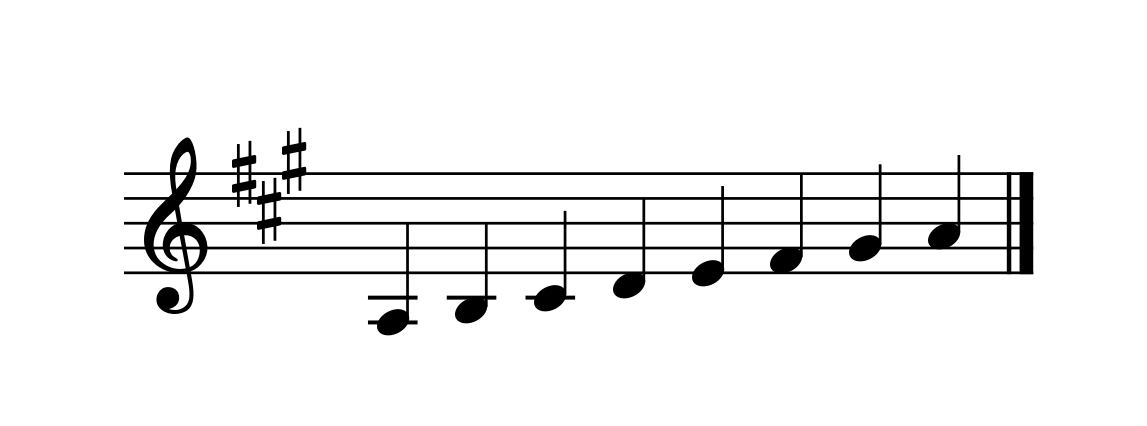
\includegraphics[width=.9\textwidth]{figs/escala.png}
            \end{figure}
            \vspace{-1cm}
            \begin{figure}
                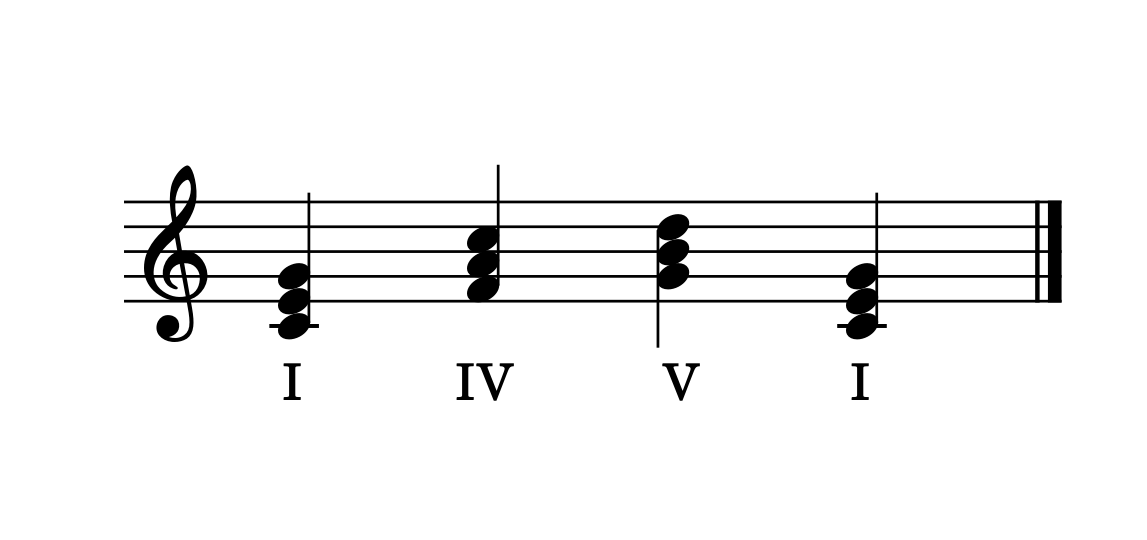
\includegraphics[width=.9\textwidth]{figs/acorde.png}
            \end{figure}
        \end{column}
    \end{columns}
\end{frame}

\subsection{Tonalidades Próximas}
\begin{frame}{Fundamentos Teóricos}{Tonalidades Próximas}
    \begin{columns}[]
        \begin{column}{.5\textwidth}
            \begin{itemize}
            \item Tonalidades Próximas / Afastadas
            \item Tónica
            \item Relativa
            \begin{itemize}
                \item Maior
                \item Menor
            \end{itemize}
            \item Dominante
            \item Sub-Dominante e Relativas
            \end{itemize}
        \end{column}
        \begin{column}{.5\textwidth}
            \begin{figure}
                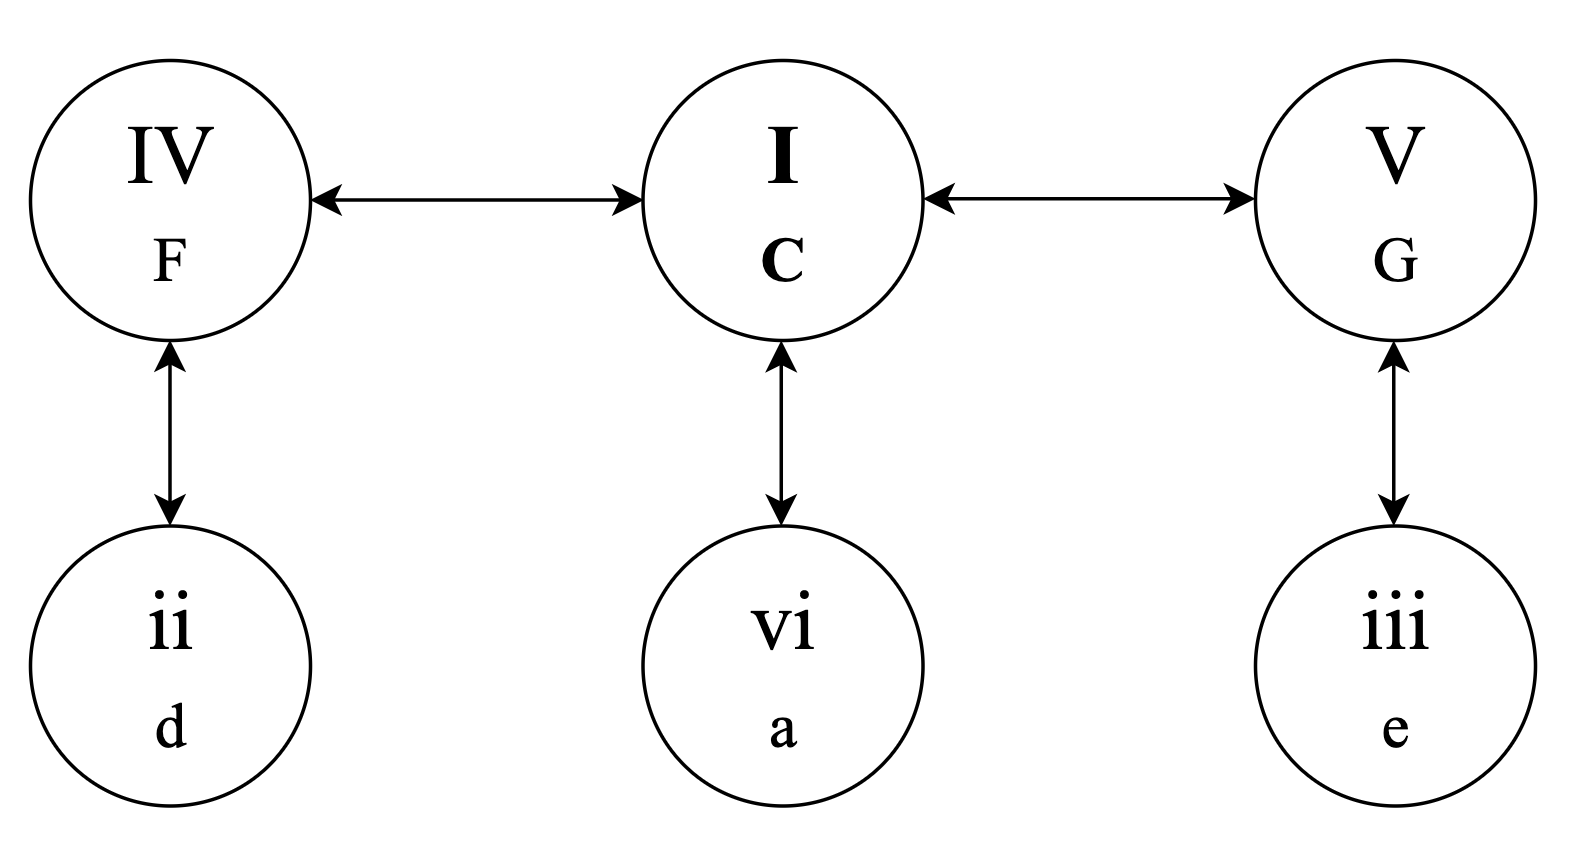
\includegraphics[width=.9\textwidth]{figs/modulacoes.png}
            \end{figure}
        \end{column}
    \end{columns}
\end{frame}

\subsection{Técnicas de Identificação}
\begin{frame}{Fundamentos Teóricos}{Técnicas de Identificação}
    \begin{columns}[]
        \begin{column}{.4\textwidth}
            \begin{itemize}
            \item Cifra
            \item Alterações (Sustenido e bemol)
            \item Progressões Harmónicas - Cadências
            \end{itemize}
        \end{column}
        \begin{column}{.6\textwidth}
            \begin{figure}
                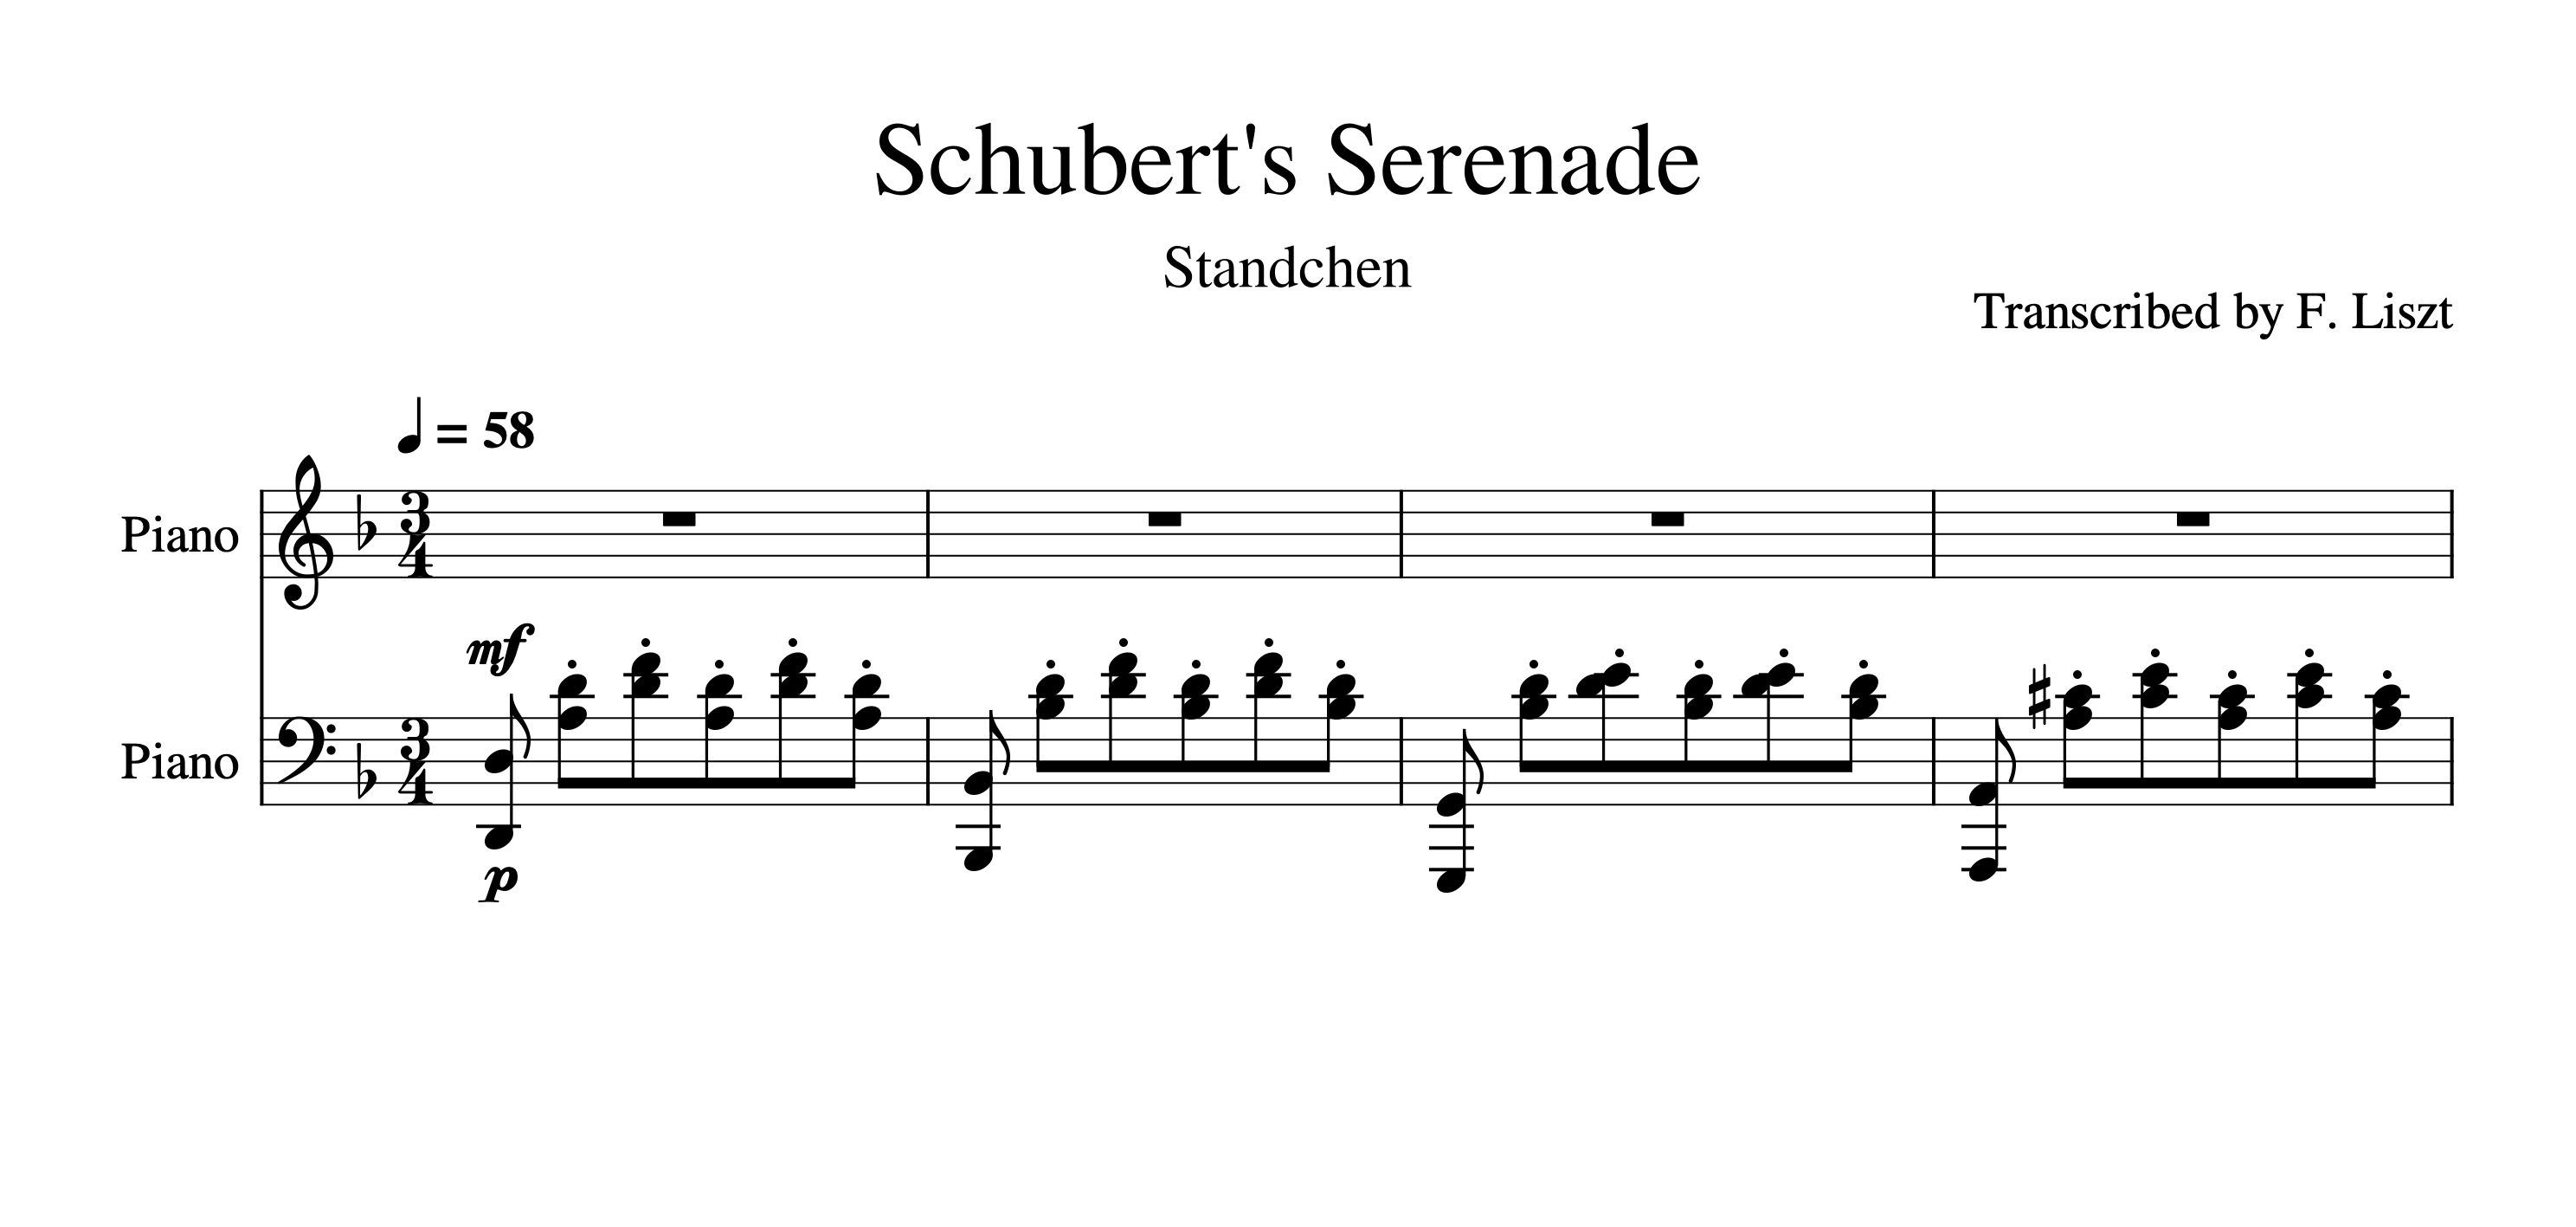
\includegraphics[width=.95\textwidth]{figs/schubert.png}
            \end{figure}
        \end{column}
    \end{columns}
\end{frame}
